\documentclass{article}
\usepackage{graphicx}
\usepackage[top=6cm, headheight=12cm]{geometry} % Adjust top margin and headheight as needed
\usepackage{fancyhdr}
\usepackage{multicol}

% Set up the page style
\pagestyle{fancy}
\fancyhf{} % Clear all header and footer fields
% \fancyfoot[C]{%
%     \begin{tabular}{@{}c@{}} % Align text elements in a row
%         Vaia Labor Tracker App \\
%         %\noindent
%         %\rule{\linewidth}{0.7pt}\\
%         Page \thepage
%     \end{tabular}%
% }

\fancyfoot[C]{\vspace{0.1cm}\hrulefill\ Vaia Labor Tracker App \hrulefill\\Page \thepage} % Custom footer

\renewcommand{\headrulewidth}{0pt} % Remove header line

% Set the header content with adjusted image height and patient information
\fancyhead[C]{%
    \begin{minipage}[b][12cm][c]{\textwidth}
        \vfill
        \centering
        
\includegraphics[width=\textwidth, height=2cm]{Imagenes/vaia_header.png} 
        \begin{multicols}{2}
            \raggedright
            Patient: <<patientName>> \\
            Date: <<date>> \\
            Age: <<patientAge>> \\
            Weeks pregnant: <<weeksPregnant>>
        \end{multicols}
        \noindent % Prevents paragraph indentation
        \rule{\linewidth}{0.7pt}
    \end{minipage}%
}



\begin{document}

\begin{center}
    \textbf{\LARGE{Contractions Report}}
\end{center}

\vspace{12pt}

\textbf{\Large{Contractions information}}

\vspace{7pt}

Duration: <<durationValue>>

\vspace{2pt}

Frequency: <<frequencyValue>>

\vspace{2pt}

Intensity: <<intensityValue>>

\vspace{2pt}

Number of contractions: <<numContractions>>

\vspace{20pt}

\textbf{\Large{Measurement information}}

\vspace{7pt}

Duration: <<measurementDuration>>

\begin{figure}[h]
    \centering
    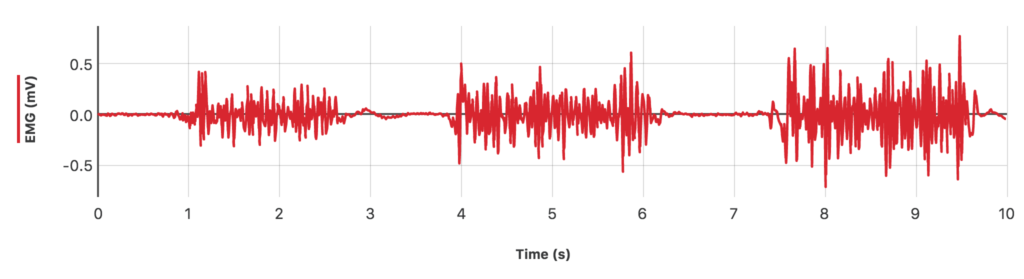
\includegraphics[width=\textwidth]{Imagenes/emg_signal.png}
    \label{fig:enter-label}
\end{figure}


\end{document}
